\documentclass{article}

\usepackage{fullpage}
\usepackage[utf8]{inputenc} % allow utf-8 input
\usepackage[T1]{fontenc}    % use 8-bit T1 fonts
\usepackage{hyperref}       % hyperlinks
\usepackage{url}            % simple URL typesetting
\usepackage{booktabs}       % professional-quality tables
\usepackage{amsmath}
\usepackage{amssymb}
\usepackage{amsfonts}       % blackboard math symbols
\usepackage{mathtools}
\usepackage{nicefrac}       % compact symbols for 1/2, etc.
\usepackage{microtype}      % microtypography
\usepackage{algorithm}
\usepackage{algpseudocode}
\usepackage{graphicx}
\usepackage{float}
\usepackage{caption}
\usepackage{outlines}
\usepackage{tikz}
\usepackage{dsfont}
\usepackage{empheq}
\usepackage{xfrac}
\usepackage{enumitem}
%\usepackage{geometry}
%\geometry{margin=1.5in}

\usetikzlibrary{bayesnet,positioning}

\newcommand{\nth}{^{\text{th}}}
\newcommand{\len}{\text{len}}
\newcommand{\indicator}{\mathds{1}}
\newcommand{\hackystatei}[1]{\State \parbox[t]{\dimexpr\linewidth-\algorithmicindent}{#1\strut}}
\newcommand{\hackystateii}[1]{\State \parbox[t]{\dimexpr\linewidth-\algorithmicindent-\algorithmicindent}{#1\strut}}

%\allowdisplaybreaks

\title{A Simple Hierarchical Topic Model}

\author{
  Andrew Leverentz \\
  \texttt{aleveren@eng.ucsd.edu} \\
}

\date{}

\begin{document}

\maketitle

%\begin{abstract}
% TODO
%\end{abstract}

%%%%%%%%%%%%%%%%%%%%%%%%%%%%%%%%
%\section{Introduction}

Several probabilistic models have been proposed for learning hierarchies of topics based from a corpus of text documents.
These include: the Nested Chinese Restaurant Process (NCRP), the Nested Hierarchical Dirichlet Process (NHDP), and Hierarchical Pachinko Allocation Modeling (HPAM).
These models are quite flexible and expressive, but it can be difficult to train these models efficiently.
This paper proposes a model which is capable of learning hierarchies of topics, but using a relatively simple framework for the sake of computational efficiency.

\section{Latent Dirichlet Allocation}

The model we propose is a fairly straightforward extension of Latent Dirichlet Allocation (LDA), which we describe first.
In LDA, we use a bag-of-words assumption, and documents are assumed to be generated according to the following process:
\begin{outline}
\1 Let $K$ be the number of distinct topics assumed to be present in the corpus.
\1 Let $\mathcal V$ be the vocabulary used by the corpus.
\1 For each topic $k \in \{1, \ldots, K\}$, draw a distribution over $\mathcal V$ according to a Dirichlet:
\[ \theta_k \sim \text{Dirichlet}(\alpha^{(\theta)}). \]
\1 For each document $d \in \{1, \ldots, D\}$:
  \2 Draw a distribution over topics according to a Dirichlet:
  \[ \phi_d \sim \text{Dirichlet}(\alpha^{(\phi)}). \]
  \2 Let $N_d$ be the number of words observed in document $d$.
  \2 For each word-slot $n \in \{1, \ldots, N_d\}$:
    \3 Draw a topic according to the probabilities in $\phi_d$.  That is,
    \[ z_{d,n} \sim \text{Categorical}(\phi_d). \]
    \3 Draw a vocabulary word according to the probabilities in $\theta_{z_{d,n}}$.  That is,
    \[ t_{d,n} \sim \text{Categorical}(\theta_{z_{d,n}}). \]
\end{outline}

The plate diagram for this model is shown in Figure~\ref{fig:plate-lda}.

%%%%
\begin{figure}[htb]
%
\centering
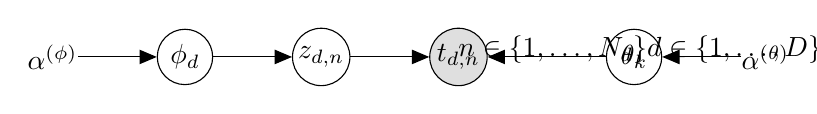
\begin{tikzpicture}
\node[obs] (t) {$t_{d,n}$};
\node[latent, right=1.5cm of t] (theta) {$\theta_k$};
\node[latent, left=of t] (z) {$z_{d,n}$};
\node[latent, left=of z] (phi) {$\phi_d$};
\node[const, right=of theta] (alphaTheta) {$\alpha^{(\theta)}$};
\node[const, left=of phi] (alphaPhi) {$\alpha^{(\phi)}$};

\edge{alphaTheta}{theta};
\edge{phi}{z};
\edge{alphaPhi}{phi};
\edge{theta}{t};
\edge{z}{t};

\centeredPlate{word-plate}{(t)(z)}{$n \in \{1, \ldots, N_d\}$};
\centeredPlate{doc-plate}{(word-plate)(phi)}{$d \in \{1, \ldots, D\}$};
\centeredPlate{topic-plate}{(theta)}{$k \in \{1, \ldots, K\}$};
\end{tikzpicture}
%
\caption{Plate diagram for the LDA model}
\label{fig:plate-lda}
\end{figure}
%%%%

\section{A Simple Hierarchical Topic Model}

We propose a model that is in many respects similar to LDA, but in which the topics are arranged into a finite, fixed-depth tree.
Furthermore, the probability of selecting a topic depends on its position in the tree.
Rather than merely selecting per-document mixtures of topics from a flat collection of topics, we first select per-document distributions over the leaves of the tree.
We also select per-document distributions over the available depths in the tree.
Together, a distribution over leaves and a distribution over depths defines a distribution over nodes.
This distribution over nodes has the property that when a document contains a mixture of two distinct leaves, it will also contain a mixture of any nodes that are common ancestors of both leaves.

The generative process for this model is
\begin{outline}
\1 Let $\mathcal T$ be a finite tree with fixed depth (i.e., all leaves appear at some constant depth $m$).
\1 Let $\mathcal V$ be the vocabulary used by the corpus.
\1 For each node $r \in \mathcal T$, draw a distribution over $\mathcal V$ according to a Dirichlet:
\[ \theta_r \sim \text{Dirichlet}(\alpha^{(\theta)}). \]
\1 For each document $d \in \{1, \ldots, D\}$:
  \2 Draw a distribution over the leaves of $\mathcal T$ according to a Dirichlet:
  \[ \lambda_d \sim \text{Dirichlet}(\alpha^{(\lambda)}). \]
  \2 Draw a distribution over the depths of $\mathcal T$ according to a Dirichlet:
  \[ \phi_d \sim \text{Dirichlet}(\alpha^{(\phi)}). \]
  \2 Let $N_d$ be the number of words observed in document $d$.
  \2 For each word-slot $n \in \{1, \ldots, N_d\}$:
    \3 Draw a leaf according to the probabilities in $\lambda_d$.  That is,
    \[ \ell_{d,n} \sim \text{Categorical}(\lambda_d). \]
    \3 Draw a depth according to the probabilities in $\phi_d$.  That is,
    \[ z_{d,n} \sim \text{Categorical}(\phi_d). \]
    \3 Let $r_{d,n} = \ell_{d,n}[1:z_{d,n}]$ represent the node at depth $z_{d,n}$ along the path from the root to the leaf $\ell_{d,n}$.  (Here, we allow $z_{d,n}$ to be $0$, corresponding to the root node.)
    \3 Draw a vocabulary word according to the probabilities in $\theta_{r_{d,n}}$.  That is,
    \[ t_{d,n} \sim \text{Categorical}(\theta_{r_{d,n}}). \]
\end{outline}

The plate diagram for this model is shown in Figure~\ref{fig:plate-simple}.

%%%%
\begin{figure}[htb]
%
\centering
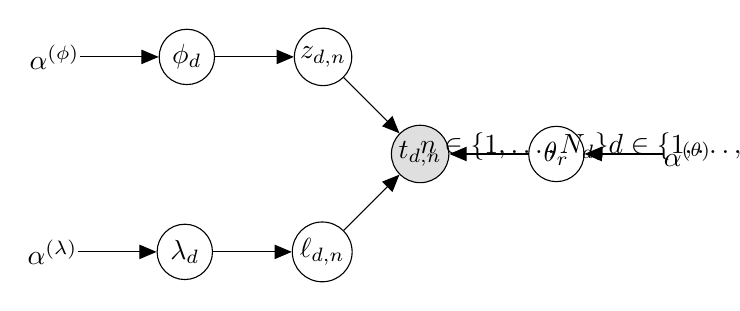
\begin{tikzpicture}
\node[obs] (t) {$t_{d,n}$};
\node[latent, right=of t] (theta) {$\theta_r$};
\node[latent, above left=of t] (z) {$z_{d,n}$};
\node[latent, below left=of t] (l) {$\ell_{d,n}$};
\node[latent, left=of z] (phi) {$\phi_d$};
\node[latent, left=of l] (lambda) {$\lambda_d$};
\node[const, right=of theta] (alphaTheta) {$\alpha^{(\theta)}$};
\node[const, left=of phi] (alphaPhi) {$\alpha^{(\phi)}$};
\node[const, left=of lambda] (alphaLambda) {$\alpha^{(\lambda)}$};

\edge{alphaTheta}{theta};
\edge{phi}{z};
\edge{alphaPhi}{phi};
\edge{theta}{t};
\edge{z}{t};
\edge{l}{t};
\edge{lambda}{l};
\edge{alphaLambda}{lambda};

\centeredPlate{word-plate}{(t)(z)(l)}{$n \in \{1, \ldots, N_d\}$};
\centeredPlate{doc-plate}{(word-plate)(phi)(lambda)}{$d \in \{1, \ldots, D\}$};
\centeredPlate{topic-plate}{(theta)}{$r \in \mathcal T$};
\end{tikzpicture}
%
\caption{Plate diagram for the Simple Hierarchical Topic Model}
\label{fig:plate-simple}
\end{figure}
%%%%

\section{Variational Inference}

\newcommand{\rPath}{{r \in \mathcal T}}
\newcommand{\vVocab}{{v \in \mathcal V}}
\newcommand{\iLeaf}{{i \in \mathcal L(\mathcal T)}}
\newcommand{\kDepth}{{k = 0}^{m}}
\newcommand{\kDepthSet}{{k \in \{0, \ldots, m\}}}
\newcommand{\nWordSlot}{{n = 1}^{N_d}}
\newcommand{\dDoc}{{d = 1}^D}
\newcommand{\softmax}{\mathop{\text{softmax}}}

This model can be trained using stochastic variational inference.
To derive the variational updates, we first express the log joint probability of the model:
\begin{align}
\MoveEqLeft
\log p(\{\theta_r\}, \{\lambda_d\}, \{\phi_d\}, \{\ell_{d,n}\}, \{z_{d,n}\}, \{t_{d,n}\}) \\
={}& \phantom{{}+{}} \sum_\rPath \log p(\theta_r) + \sum_\dDoc \log p(\lambda_d) + \sum_\dDoc \log p(\phi_d) \\
&+ \sum_\dDoc \sum_\nWordSlot \log p(\ell_{d,n} \mid \lambda_d) + \sum_\dDoc \sum_\nWordSlot \log p(z_{d,n} \mid \phi_d) \nonumber \\
&+ \sum_\dDoc \sum_\nWordSlot \log p(t_{d,n} \mid \{\theta_r\}, \ell_{d,n}, z_{d,n}) \nonumber \\
={}& \text{constant} + \sum_\rPath \sum_\vVocab (\alpha^{(\theta)}_v - 1) \log \theta_{r,v} \\
&+ \sum_\dDoc \sum_\iLeaf (\alpha^{(\lambda)}_i - 1) \log \lambda_{d,i} \nonumber \\
&+ \sum_\dDoc \sum_\kDepth (\alpha^{(\phi)}_k - 1) \log \phi_{d,k} \nonumber \\
&+ \sum_\dDoc \sum_\nWordSlot \sum_\iLeaf \indicator[\ell_{d,n} = i] \log \lambda_{d,i} \nonumber \\
&+ \sum_\dDoc \sum_\nWordSlot \sum_\kDepth \indicator[z_{d,n} = k] \log \phi_{d,k} \nonumber \\
&+ \sum_\dDoc \sum_\nWordSlot \sum_\iLeaf \sum_\kDepth \sum_\rPath \sum_\vVocab \indicator[r = i[1:k]] \indicator[z_{d,n} = k] \indicator[\ell_{d,n} = i] \indicator[t_{d,n} = v] \log \theta_{r,v}. \nonumber
\end{align}
Here, $\mathcal L(\mathcal T)$ denotes the leaves of $\mathcal T$, and $m$ is the depth of $\mathcal T$.

Next, we seek a variational distribution $q$ which approximates the posterior distribution of the latent variables given the observed data, $\{t_{d,n}\}$, and which takes the following form:
\begin{align}
\MoveEqLeft
q(\{\theta_r\}, \{\lambda_d\}, \{\phi_d\}, \{\ell_{d,n}\}, \{z_{d,n}\}) \\
={}& \prod_\rPath \text{Dirichlet}(\theta_r \mid \mu^{(\theta)}_r)
\cdot \prod_\dDoc \text{Dirichlet}(\lambda_d \mid \mu^{(\lambda)}_d)
\cdot \prod_\dDoc \text{Dirichlet}(\phi_d \mid \mu^{(\phi)}_d) \nonumber \\
&\cdot \prod_\dDoc \prod_\nWordSlot \text{Categorical}(\ell_{d,n} \mid \mu^{(\ell)}_{d,n})
\cdot \prod_\dDoc \prod_\nWordSlot \text{Categorical}(z_{d,n} \mid \mu^{(z)}_{d,n}). \nonumber
\end{align}
The variables named $\mu$ are known as variational parameters, and we wish to find the value for these variational parameters which minimizes the KL divergence between $q$ and the true posterior.
Since we are assuming that $q$ can be expressed as a product of univariate factors, this formulation corresponds to the \emph{mean-field approximation}.

The variational updates for this model involve a straightforward application of stochastic variational inference.
In this context, the per-document random variables are considered ``local,'' and the topic vectors $\{\theta_r\}$ are considered ``global.''
The local variational updates correspond to coordinate-ascent update rules:
\begin{align}
\mu^{(\lambda)}_d
&\gets \left( \alpha^{(\lambda)}_i + \sum_\nWordSlot E_q[\indicator[\ell_{d,n} = i]] \right)_\iLeaf \\
\mu^{(\phi)}_d
&\gets \left( \alpha^{(\phi)}_k + \sum_\nWordSlot E_q[\indicator[z_{d,n} = k]] \right)_\kDepthSet \\
\mu^{(\ell)}_{d,n}
&\gets \softmax_\iLeaf \left( E_q[\log \lambda_{d,i}] +
\sum_\kDepth \sum_\rPath \sum_\vVocab
\indicator[r = i[1:k]] \cdot \indicator[t_{d,n} = v] \cdot E_q[\indicator[z_{d,n} = k]] \cdot E_q[\log \theta_{r,v}]
\right) \\
\mu^{(z)}_{d,n}
&\gets \softmax_\kDepthSet \left( E_q[\log \phi_{d,k}] +
\sum_\iLeaf \sum_\rPath \sum_\vVocab
\indicator[r = i[1:k]] \cdot \indicator[t_{d,n} = v] \cdot E_q[\indicator[\ell_{d,n} = i]] \cdot E_q[\log \theta_{r,v}]
\right)
\end{align}
Here, $E_q$ denotes that the expectation is to be computed under the assumption that all latent variables are distributed according to the current value of $q$ (which, in turn, is determined by the current value of the variational parameters $\mu$).
Furthermore, softmax is defined as
\begin{align}
\softmax_{x \in S} f(x)
&= \left( \frac{\exp(f(x))}{\sum_{y \in S} \exp(f(y))} \right)_{x \in S}
\end{align}

For this model, we have:
\begin{align}
E_q[\log \theta_{r,v}]
&= \psi \left( \mu^{(\theta)}_{r,v} \right) - \psi \left( \sum_{v' \in \mathcal V} \mu^{(\theta)}_{r,v'} \right) \\
E_q[\log \lambda_{d,i}]
&= \psi \left( \mu^{(\lambda)}_{d,i} \right) - \psi \left( \sum_{i' \in \mathcal L(\mathcal T)} \mu^{(\lambda)}_{d,i'} \right) \\
E_q[\log \phi_{d,k}]
&= \psi \left( \mu^{(\phi)}_{d,k} \right) - \psi \left( \sum_{k' = 0}^m \mu^{(\phi)}_{d,k'} \right) \\
E_q[\indicator[z_{d,n} = k]]
&= \mu^{(z)}_{d,n,k} \\
E_q[\indicator[\ell_{d,n} = i]]
&= \mu^{(\ell)}_{d,n,i}
\end{align}
Here, $\psi$ is the digamma function.

The global variational updates are performed on mini-batches of documents.
Let $\rho_t$ denote a decaying schedule of step-sizes, and let $B$ denote a randomly selected subset of $\{1, \ldots, D\}$.
Then, at the $t\nth$ step, we have
\begin{align}
\mu^{(\theta)}_r
&\gets
(1-\rho_t) \mu^{(\theta)}_r
+
\rho_t
\left[ \alpha^{(\theta)} + \frac{D}{|B|} \left( \beta_{r,v} \right)_\vVocab \right]
\shortintertext{where}
\beta_{r,v} &= \sum_{d \in B} \sum_\nWordSlot \sum_\iLeaf \indicator[t_{d,n} = v] \cdot \indicator[r \text{ is a prefix of } i] \cdot E_q[\indicator[z_{d,n} = \len(r)]] \cdot E_q[\indicator[\ell_{d,n} = i]]
\end{align}

We repeatedly apply these variational updates until we reach convergence.
To assess the convergence of this algorithm, we can compute the evidence lower bound (ELBO) as follows:
\begin{align}
\text{ELBO}
={}& \phantom{{}-{}} E_q[\log p(\{\theta_r\}, \{\lambda_d\}, \{\phi_d\}, \{\ell_{d,n}\}, \{z_{d,n}\}, \{t_{d,n}\})] \\
& - E_q[\log q(\{\theta_r\}, \{\lambda_d\}, \{\phi_d\}, \{\ell_{d,n}\}, \{z_{d,n}\})] \nonumber \\
={}& \phantom{{}+{}} \sum_\rPath \sum_\vVocab \left(\alpha^{(\theta)}_v - \mu^{(\theta)}_{r,v}\right) E_q[\log \theta_{r,v}] \\
&- |\mathcal T| \sum_\vVocab \log \Gamma\left( \alpha^{(\theta)}_{v} \right) + |\mathcal T| \log \Gamma\left( \sum_\vVocab \alpha^{(\theta)}_{v} \right)
 + \sum_\rPath \sum_\vVocab \log \Gamma\left( \mu^{(\theta)}_{r,v} \right) - \sum_\rPath \log \Gamma\left( \sum_\vVocab \mu^{(\theta)}_{r,v} \right) \nonumber \\
&+ \sum_\dDoc \sum_\iLeaf \left(\alpha^{(\lambda)}_i - \mu^{(\lambda)}_{d,i}\right) E_q[\log \lambda_{d,i}] \nonumber \\
&- D \sum_\iLeaf \log \Gamma\left( \alpha^{(\lambda)}_{i} \right) + D \log \Gamma\left( \sum_\iLeaf \alpha^{(\lambda)}_{i} \right)
 + \sum_\dDoc \sum_\iLeaf \log \Gamma\left( \mu^{(\lambda)}_{d,i} \right) - \sum_\dDoc \log \Gamma\left( \sum_\iLeaf \mu^{(\lambda)}_{d,i} \right) \nonumber \\
&+ \sum_\dDoc \sum_\kDepth \left(\alpha^{(\phi)}_k - \mu^{(\phi)}_{d,k}\right) E_q[\log \phi_{d,k}] \nonumber \\
&- D \sum_\kDepth \log \Gamma\left( \alpha^{(\phi)}_{k} \right) + D \log \Gamma\left( \sum_\kDepth \alpha^{(\phi)}_{k} \right)
 + \sum_\dDoc \sum_\kDepth \log \Gamma\left( \mu^{(\phi)}_{d,k} \right) - \sum_\dDoc \log \Gamma\left( \sum_\kDepth \mu^{(\phi)}_{d,k} \right) \nonumber \\
&+ \sum_\dDoc \sum_\nWordSlot \sum_\iLeaf E_q[\indicator[\ell_{d,n} = i]] \left(E_q[\log \lambda_{d,i}] - \log \mu^{(\ell)}_{d,n,i}\right) \nonumber \\
&+ \sum_\dDoc \sum_\nWordSlot \sum_\kDepth E_q[\indicator[z_{d,n} = k]] \left(E_q[\log \phi_{d,k}] - \log \mu^{(z)}_{d,n,k}\right) \nonumber \\
&+ \sum_\dDoc \sum_\nWordSlot \sum_\iLeaf \sum_\kDepth \sum_\rPath \sum_\vVocab \indicator[r = i[1:k]] E_q[\indicator[z_{d,n} = k]] E_q[\indicator[\ell_{d,n} = i]] \indicator[t_{d,n} = v] E_q[\log \theta_{r,v}]. \nonumber
\end{align}

\section{Gibbs Sampling}

By again using computations that involve the complete conditionals of this model, we can derive a Gibbs sampling algorithm.
The update rules are as follows:
\begin{align}
\phi_d &\gets \text{sample from Dirichlet}(\gamma^{(\phi)}_d) \\
\lambda_d &\gets \text{sample from Dirichlet}(\gamma^{(\lambda)}_d) \\
\theta_r &\gets \text{sample from Dirichlet}(\gamma^{(\theta)}_r) \\
z_{d,n} &\gets \text{sample from Categorical}(\gamma^{(z)}_{d,n}) \\
\ell_{d,n} &\gets \text{sample from Categorical}(\gamma^{(\ell)}_{d,n})
\end{align}
%
Here, the parameters $\gamma$ for the complete conditionals are given by
\begin{align}
\gamma^{(\phi)}_d
&= \left( \alpha^{(\phi)}_k + \sum_\nWordSlot \indicator[z_{d,n} = k] \right)_\kDepthSet \\
%
\gamma^{(\lambda)}_d
&= \left( \alpha^{(\lambda)}_i + \sum_\nWordSlot \indicator[\ell_{d,n} = i] \right)_\iLeaf \\
%
\gamma^{(\theta)}_r
&= \left( \alpha^{(\theta)}_v + \sum_\dDoc \sum_\nWordSlot \indicator[t_{d,n} = v] \cdot \indicator[r = \ell_{d,n}[1:z_{d,n}]] \right)_\vVocab \\
%
\gamma^{(z)}_{d,n}
&= \softmax_\kDepthSet \left( \log \phi_{d,k} + \log \theta_{\ell_{d,n}[1:k], t_{d,n}} \right) \\
%
\gamma^{(\ell)}_{d,n}
&= \softmax_\iLeaf \left( \log \lambda_{d,i} + \log \theta_{i[1:z_{d,n}], t_{d,n}} \right)
\end{align}

Note that the update rule for $\theta_r$ is particularly slow, since the computation of $\gamma^{(\theta)}_r$ involves a pass through the entire dataset.

% TODO: can we derive a Collapsed Gibbs sampler?

%%%%%%%%%%%%%%%%%%%%%%%%%%%%%%%%
%\clearpage
%\nocite{*}
%%\bibliographystyle{plainnat}
%\bibliographystyle{plain}
%\bibliography{bibliography}

\end{document}
